In zahlreichen Experimenten zur Bestimmung von Winkeln und Bindungsabständen wurde belegt, dass ein Methanmolekül die Form eines Tetraeders besitzt. Alle Bindungen sind somit identisch.
Die Berechnung eines Methanmoleküls zeigte einen Unterschied zwischen den Energieniveaus der vier höchsten besetzten Molekülorbitale. Die Abbildung \ref{EnergieniveausMethan} verdeutlicht dies.

\begin{dsafigure}
 \centering
 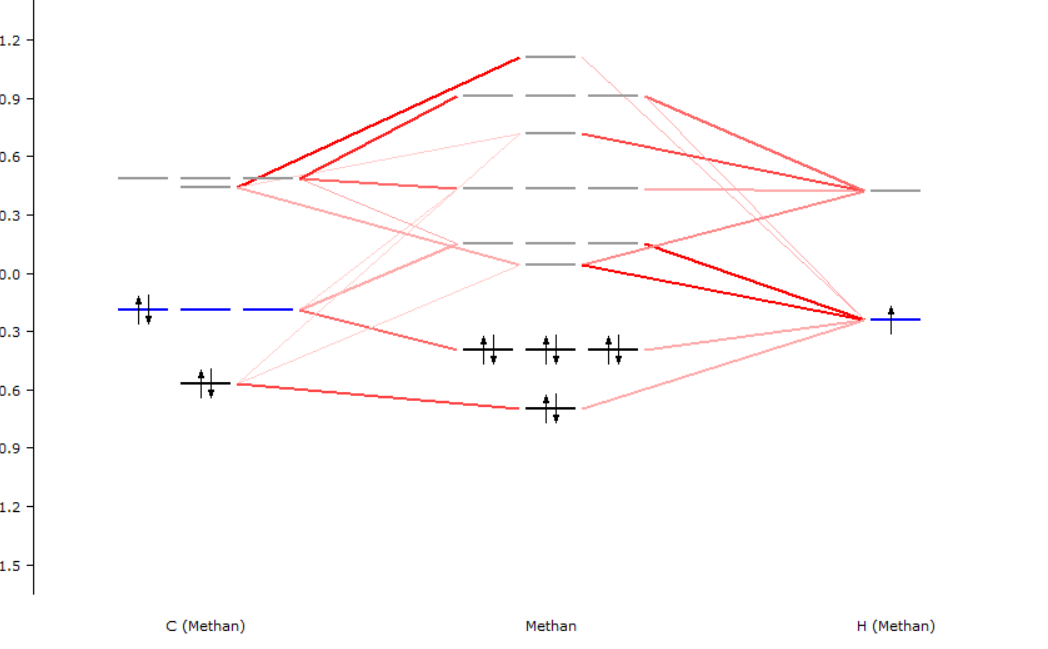
\includegraphics[width=\columnwidth]{LevelsMethan.png}
 \caption{Energieniveaus des Methanmoleküls \cite{ADF2017authors}.}
 \label{EnergieniveausMethan}
\end{dsafigure}

Links sind die Atomorbitale eines Kohlenstoffatoms und rechts die Atomorbitale eines Wasserstoffatoms abgebildet. In der Mitte sind dann die Molekülorbitale des Methanmoleküls dargestellt. Die horizontalen Linien repräsentieren die Energieniveaus der verschiedenen Orbitale. Dabei wird deutlich, dass ein Molekülorbital eine geringere Energie als die übrigen drei der vier höchsten besetzten Molekülorbitale besitzt. 
Es zeigt sich ein Unterschied zwischen dem Modell der Hybridorbitale und der von ADF genutzten Molekülorbitaltheorie, durch die man auch quantitative Informationen wie die Energien erhält. Das Modell der Hybridorbitale hingegen definiert die Energien nicht, sondern liefert qualitative Aussagen zur Geometrie und Bindungsverhältnissen. Hybridorbitale resultieren bloß aus der Anpassung der Atomorbitalbasis an die Tertaederstruktur des Moleküls. Für die Molekülorbitale werden hingegen die Energien einzelner Elektronen optimiert. 
Es handelt sich also um zwei unterschiedliche Betrachtungsweisen.
Insgesamt beschreiben beide Modelle die Struktur des Methanmoleküls als Tetraeder. In Abbildung \ref{OrbitalMethan} ist eins der drei HOMOs dargestellt.

\begin{dsafigure}
 \centering
 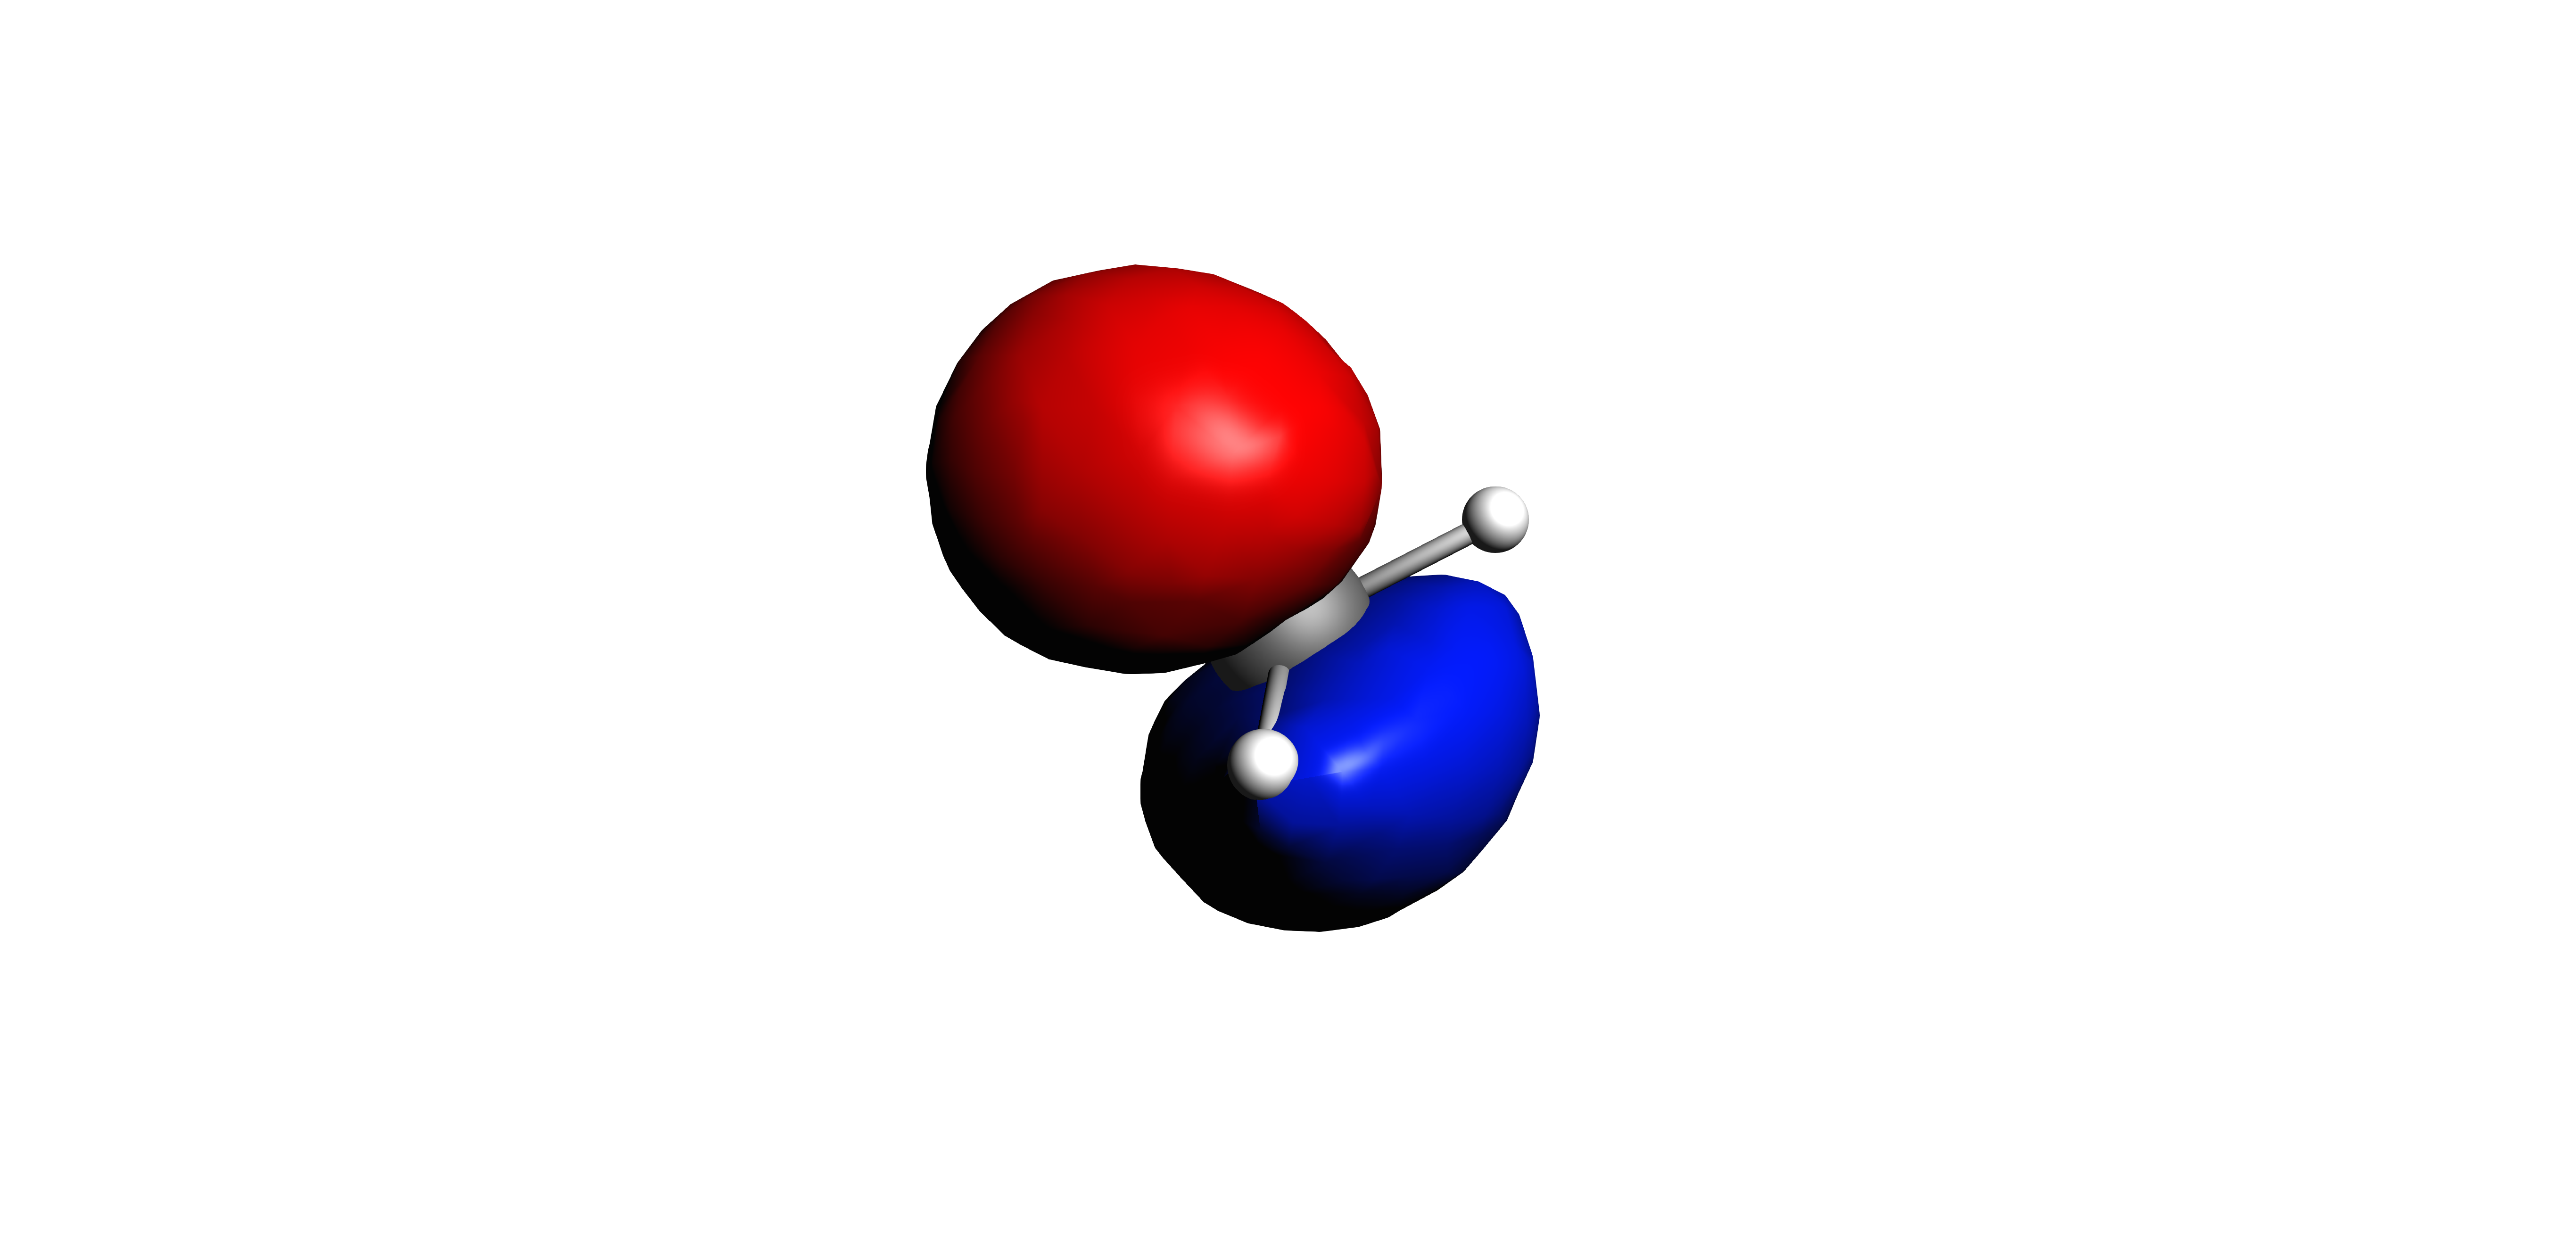
\includegraphics[scale=0.04]{MethanA5.png}
 \caption{Eines der drei HOMOs eines Methanmoleküls \cite{ADF2017authors}.}
 \label{OrbitalMethan}
\end{dsafigure}
